\section{Algoritmy}\label{sec:algorithms}

Počas vývoja výpočtovej techniky sa vyvíjali aj algoritmy pre kombinatorické hry, pričom piškvorky sú jednou z nich.
Tieto algoritmy je možné rozdeliť do 2 skupín: \emph{exaktné} a \emph{heuristické}; v tejto práci je popísaný jeden
algoritmus z každej skupiny.

\subsection{MiniMax}\label{subsec:algo-minmax}

Minimax je rozhodovacie pravidlo, podľa ktorého je možné určiť nasledujúci ťah.
Jeho princíp spočíva v maximalizovaní úžitku pre cieľového hráča a minimalizovaní úžitku pre oponenta.
Pôvodne bol vyvinutý pre \emph{hru s nulovým súčtom} (angl. zero-sum), čo je termín používaný v teórii hier a vyjadruje hru, kde
rozhodnutia hráčov sa dajú ohodnotiť nenulovým číslom $v$.
Často používaná hodnota je $v=1$.
Ťah cieľového hráča je vyjadrený kladnou hodnotou ($+v$), ťah protihráča je vyjadrený zápornou hodnotou ($-v$).
Hru, ktorú hrajú hráči striedavo je možné vyjadriť pomocou postupnosti pre párny počet ťahov:

\begin{equation}
    v-v+v-v+ \dots = \sum{v-v} = \sum{0} = 0
\end{equation}

(z čoho vychádza aj názov \emph{hra s nulovým súčtom}), resp. pre nepárny počet ťahov:

\begin{equation}
    \pm v+v-v+v-v+ \dots = \pm v+\sum{v-v} = \pm v+\sum{0} = \pm v
\end{equation}

Rozhodovanie vychádza práve z tohto faktu, pričom sa snaží nájsť takú postupnosť ťahov, ktorá by bola rovná $+v$, čo
by znamenalo výhru cieľového hráča.

Samotný rozhodovací proces sa dá vyjadriť pomocou rozhodovacieho stromu vychádzajúceho z aktuálneho stavu hry.

\subsection{Umelá neurónová sieť}\label{subsec:algo-ann}

Najdôležitejšou časťou práce je vytvoriť neurónovú sieť, ktorá by mala spĺňať tieto vlastnosti:
\begin{itemize}
    \item na vstupe má byť aktuálny stav hry
    \item na výstupe má byť informácia o tom, ktoré pole je pre aktuálneho hráča najlepšie pre ďalší krok
\end{itemize}

Stav hry je reprezentovaný vektor $s_i$ pre $i=1 \dots r^d$, kde každých $r$ prvkov reprezentuje riadok hracej plochy,
resp. hracieho priestoru.
Napríklad pre rozmer 3x3 má vektor $s$ dĺžku 9 ($r^d=3^2$), prvky 1-3 reprezentujú prvý riadok, prvky 4-6 reprezentujú
druhý riadok a prvky 7-9 reprezentujú posledný riadok.
Neurónová sieť pozostáva z 3 vrstiev (vstupná, skrytá, výstupná).
Nech $x_i$ pre $i=1 \dots 3r^d$ je neurón vo vstupnej vrstve.
Za vstup do neurónovej siete je považovaný vektor hodnôt $x_1$ až $x_{3r^d}$, kde
\begin{equation}
    x_i=
    \begin{cases}
        1 & \text{ak }s_i\text{ je prázdne a } i \in \langle 1, r^d \rangle \\
        1 & \text{ak }s_{i-r^d}\text{ je }\textbf{X}\text{ a } i \in \langle r^d+1, 2r^d \rangle \\
        1 & \text{ak }s_{i-2r^d}\text{ je }\textbf{O}\text{ a } i \in \langle 2r^d+1, 3r^d \rangle \\
        0 & \text{inak}
    \end{cases}
    \quad
    \text{pre }i=1 \dots 3r^d
\end{equation}
Nech $y_j$ pre $j=1 \dots r^d$ je neurón v skrytej vrstve.
Táto vrstva zabezpečuje reprezentáciu stavu hry, na základe ktorej sa nastavujú váhy pre jednotlivé hodnoty políčok
hracej plochy.
Tieto váhy je možné označiť $w_{ij}$ pre $i=1 \dots 3r^d$, $j=1 \dots r^d$, kde index $ij$ vyjadruje váhu hodnoty
$x_i$ vstupujúcu do neurónu $y_j$.
Zo vstupnej vrstvy do skrytej vrstvy sa teda prenesú hodnoty
\begin{equation}
    \sum_{i=1}^{3r^d} w_{ij}x_{ij} \quad \text{pre } j=1 \dots r^d
\end{equation}
Posledná (skrytá) vrstva má len jeden neurón $z$, ktorý vyjadruje index $i$ vo vektore $s_i$ pre najlepší možný ťah
hráča.
Váhy zo skrytej vrstvy vstupujúce do poslednej vrstvy je možné označiť $v_j$.
Zo skrytej vrstvy do výstupnej vrstvy sa prenesú hodnoty
\begin{equation}
    \sum_{j=1}^{r^d} v_{j}y_{j}
\end{equation}
Neurónová sieť vyzerá nasledovne:

\begin{figure}[H]
    \centering
    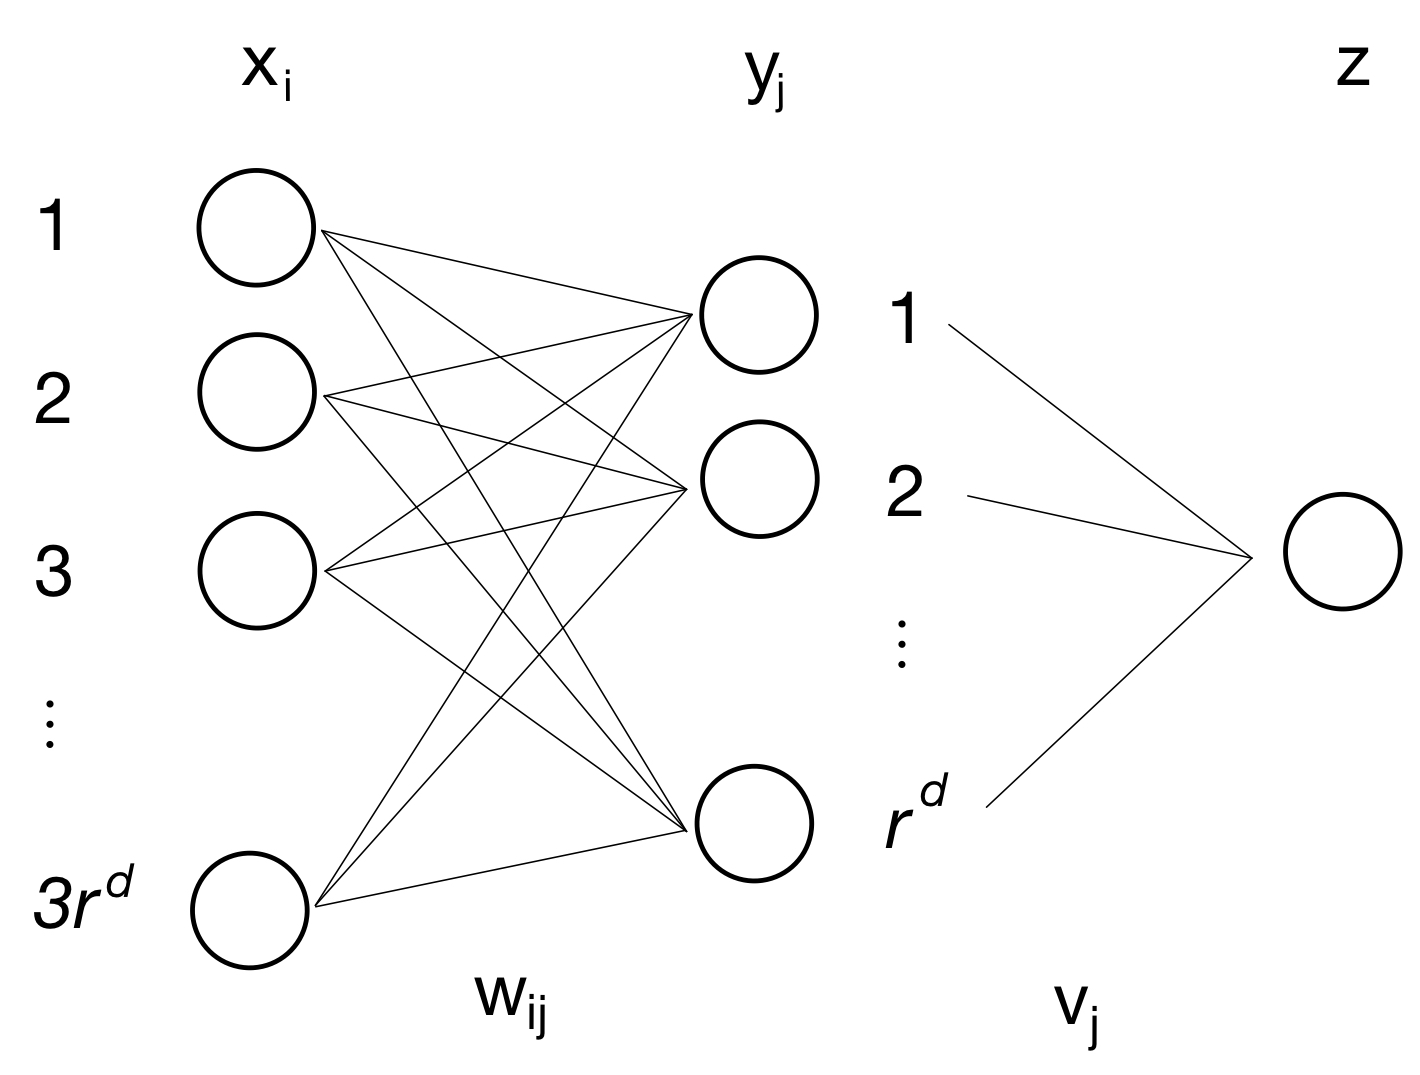
\includegraphics[width=0.5\textwidth]{images/ann.jpg}
    \caption{Návrh neurónovej siete}
\end{figure}

